\section{Introduksjon}\label{sec:intro}

Analog motorlab hadde som mål å konstruere et sett med kretser for å måle og kontrollere en servomotor. Disse kretsene var delt inn i 4 forskjellige delsystemer, en hastighetsmåler, hastighetsregulator, posisjonsmåler og posisjonsregulator, som vist i \autoref{fig:blokkdiagram}. Denne rapporten vil gå gjennom teori, metode, resultater og diskusjon for hver av delsystemene.

Utlevert til laboratoriearbeidet var et motorkort og et studentkort, motoren med takometeret og potensiometeret var koblet på et ferdig montert motorkort som ga tilgang til informasjon om motorens hastighet $\omega$, og posisjon $\theta$. Studentkortet besto av 13 operasjonsforsterkerer av typen LM741\cite{LM741} og et sett med header-pinner for å koble til motorkortet med. Operasjonsforsterkerene ble alle forsynt med $\pm${\SI{15}{\volt}}. 

Motorens hastighet kunne justeres ved å endre spenningen $V_m$ på en av pinnene på headeren. Det ble først laget et system for å måle og regulere hastighet før det ble laget et tilsvarende system for å måle og regulere posisjonen til motoren.

\begin{figure}[bh]
    \centering
    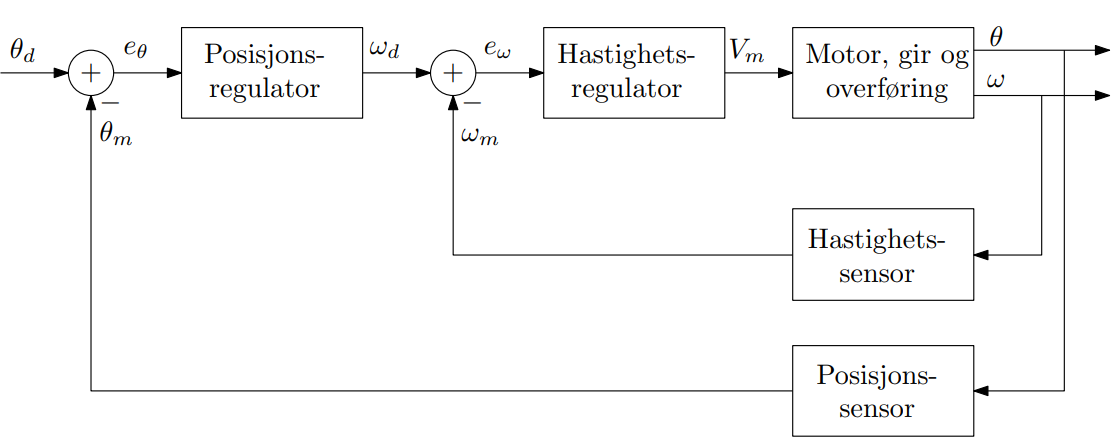
\includegraphics[width = 0.5\textwidth]{figurer/Blokkdiagram.png}
    \caption{Blokkdiagram over servomotoren. Diagrammet viser regulatorene og signalomforming. Figuren er hentet fra \cite{AnalogMotorlabbOppgaver}.}
    \label{fig:blokkdiagram}
\end{figure}
